%%%%%%%%%%%%%%%%%%%%%%%%%%%%%%%%%%%%%%%%%%%%%%%
\chapter{Introduction} \label{chap:intro}
%%%%%%%%%%%%%%%%%%%%%%%%%%%%%%%%%%%%%%%%%%%%%%%
\graphicspath{{C:/Users/Kevin/Bachelarbeit/Bachelorarbeit/01_Bachelorarbeit_LaTex/02_Figures/}}


\section{Intro}

With the ever growing market of mobile devices and the slow approach of next generation of wireless communication in form of 5G an utmost importance and interest is set on wireless communication. While in itself LTE or 4G can be explained shortly for a layman to understand there are many techniques and difficulties behind it before reaching a feasible wireless transmission. Most recently seen in the development of the 5G network with its unofficial launch date as standard communication system in 2020. (!!cite!!) In this thesis we will discuss the difficulties of transmission of data in unknown channel. A functioning channel consisting of transmitter and receiver will be built and different channel settings will be tested. Different solutions will be given to increase transmission efficiency and error rates of the system.




\begin{figure}[!htb]
    \centering
    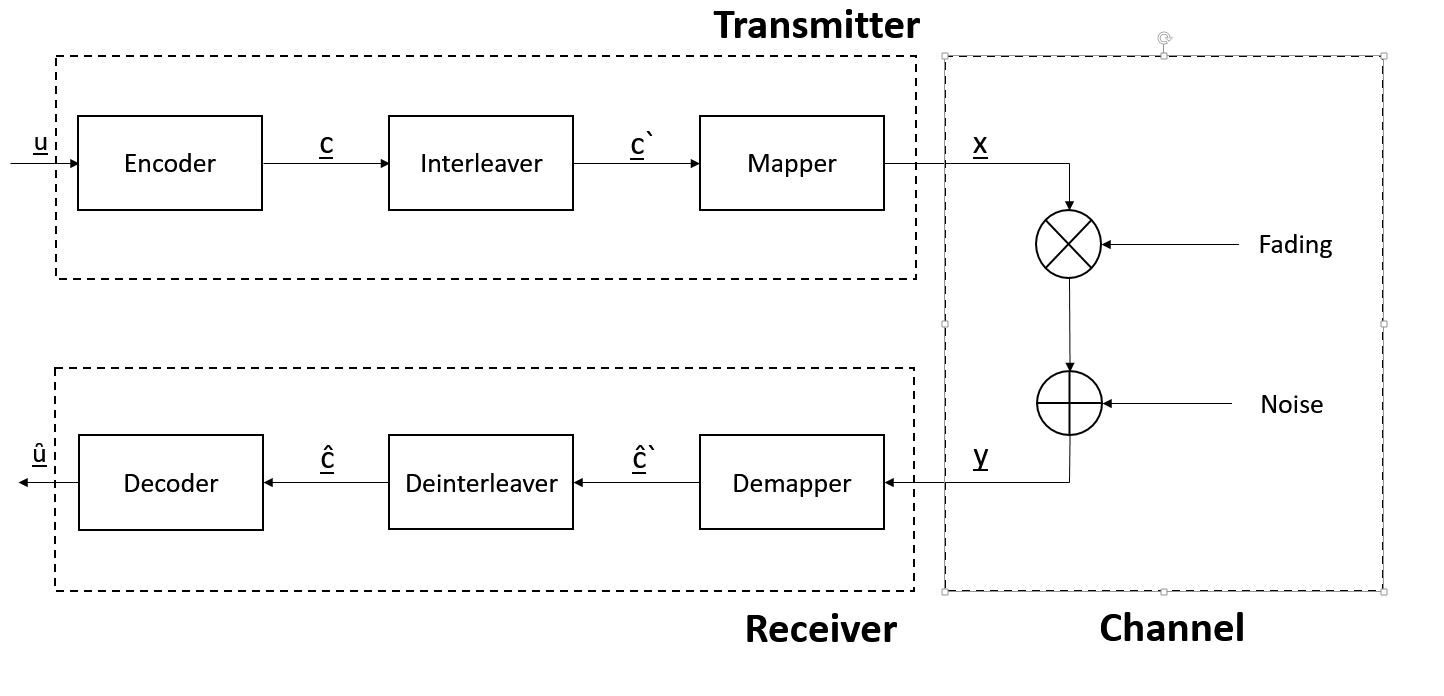
\includegraphics[width=0.8\textwidth]{Channelmodel.PNG}
    \caption{PDF $p_N(N)$ of the number N of times that the head side is up.}
    \label{fig:coin_bino}
\end{figure}



\clearpage
